\documentclass{article}

%other packages
\usepackage[a4paper]{geometry}
\usepackage{longtable}
\usepackage{wrapfig}
\setlength\parindent{0pt}
\usepackage{enumitem}
\usepackage[table,dvipsnames]{xcolor}
\usepackage{polynom}
\def\scaleint#1{\vcenter{\hbox{\scaleto[3ex]{\displaystyle\int}{#1}}}}
\usepackage{array}
\newcolumntype{C}{>{{}}c<{{}}} % for '+' and '-' symbols
\newcolumntype{R}{>{\displaystyle}r} % automatic display-style math mode 
\usepackage{tabularray}
\usepackage{dcolumn,tabularx,booktabs}
\usepackage[most]{tcolorbox}

%maths
\usepackage{mathtools}
\usepackage{amsmath}
\usepackage{amssymb}
\usepackage{amsfonts}
\usepackage{autobreak}

%tikzpicture
\usepackage{tikz}
\usepackage{scalerel}
\usepackage{pict2e}
\usepackage{tkz-euclide}
\usepackage{tikz-3dplot}
\usetikzlibrary{calc}
\usetikzlibrary{patterns,arrows.meta}
\usetikzlibrary{shadows}
\usetikzlibrary{external}
\usetikzlibrary{decorations.pathreplacing,angles,quotes}

%pgfplots
\usepackage{pgfplots}
\pgfplotsset{compat=1.18}
\usepgfplotslibrary{statistics}
\usepgfplotslibrary{fillbetween}

\pgfplotsset{
    standard/.style={
    axis line style = thick,
    trig format=deg,
    enlargelimits,
    axis x line=middle,
    axis y line=middle,
    enlarge x limits=0.15,
    enlarge y limits=0.15,
    every axis x label/.style={at={(current axis.right of origin)},anchor=north west},
    every axis y label/.style={at={(current axis.above origin)},anchor=south east}
    }
}

\begin{document}

Hyperbolic functions are just like trigonometric functions,  but for hyperbolas; that is, the sine hyperbolic and cosine hyperbolic functions output the vertical and horizontal projections respectively of the radial line which intersects the hyperbola - the area of the region enclosed by this line, the hyperbola, and the coordinate axis is half the paramater. Hyperbolas are defined as this: $x^2-y^2=a^2$.

\begin{center}
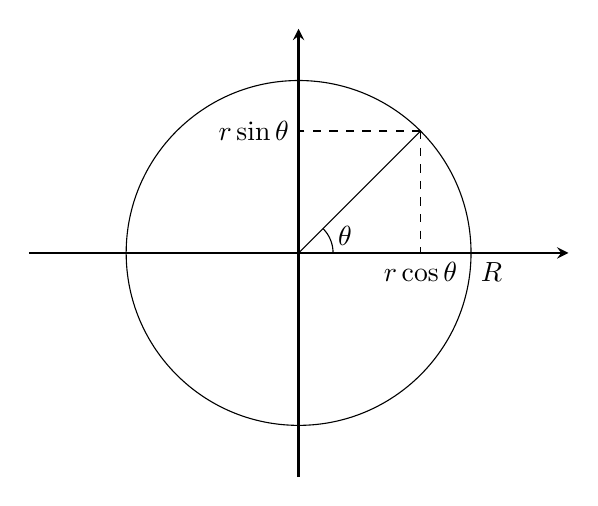
\begin{tikzpicture}
\begin{axis}[
standard,
xmin=-1, xmax=1,
ymin=-1, ymax=1,
axis equal,
xtick={\empty}, ytick={\empty}]
\draw[] (0,0) circle [radius=1];
\node[below right] at (1,0) {$R$};
\draw[] (0,0) -- (45:1);
\draw[dashed] (45:1) -- (45:1 |- 0,0) node[pos=1, below] {$r\cos\theta$};
\draw[dashed] (45:1) -- (45:1 -| 0,0) node[pos=1, left] {$r\sin\theta$};;
\draw[] (0.2,0) arc [start angle=0, end angle=45, radius=0.2];
\node[right] at (30:0.2) {$\theta$}; 
\end{axis}
\end{tikzpicture}
\hspace{20pt}
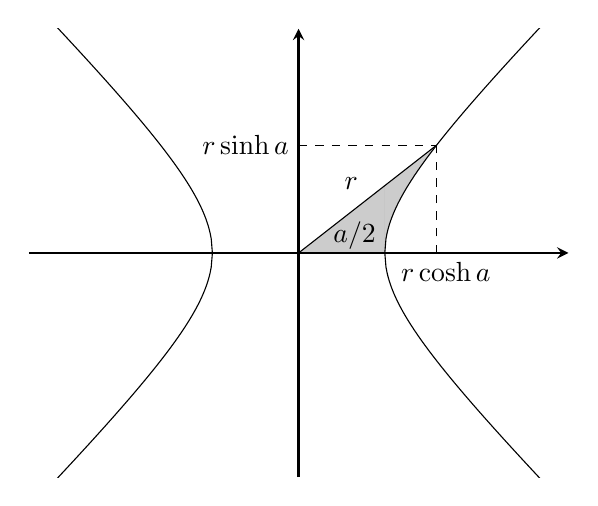
\begin{tikzpicture}
\begin{axis}[
standard,
xmin=-2, xmax=2,
ymin=-2, ymax=2,
axis equal,
xtick={\empty}, ytick={\empty}]
\addplot[samples=300,domain=1:5, name path=G] {(x^2-1)^(1/2)};
\addplot[samples=300,domain=1:5] {-(x^2-1)^(1/2)};
\addplot[samples=300,domain=-1:-5] {(x^2-1)^(1/2)};
\addplot[samples=300,domain=-1:-5] {-(x^2-1)^(1/2)};
\path[name path=H] (0,0) -- (1,0);
\draw[name path=F] (0,0) -- (1.6,1.24936) node[pos=0.5, above left] {$r$};
\addplot[fill=black, fill opacity=0.2] fill between [of=F and G, soft clip={domain=1:1.6}];
\addplot[fill=black, fill opacity=0.2] fill between [of=F and H, soft clip={domain=0:1}];
\node[] at (0.65,0.2) {$a/2$};
\draw[dashed] (0,1.24936) -- (1.6,1.24936) node[pos=0, left]{$r\sinh a$};
\draw[dashed] (1.6,0) -- (1.6,1.24936) node[pos=0, below]{$\ \ r\cosh a$};
\end{axis}
\end{tikzpicture}
\end{center}

\vspace{10pt}

And these are the relevant definitions, though they will not be on the test.

\begin{align}
\sinh x&=\frac{e^x-e^{-x}}{2}\\
\cosh x&=\frac{e^x+e^{-x}}{2}\\
\tanh x&=\frac{\sinh x}{\cosh x}\\
\coth x&=\frac{\cosh x}{\sinh x}
\end{align}

\vspace{10pt}

Then we derived a useful formula for hyperbolic tangent;

\begin{align*}
\tanh x&=\frac{e^x-e^{-x}}{e^x+e^{-x}}\\
&\overset{\div e^{-x}}{\underset{\frac{e^x}{e^{-x}}=e^{2x}}{=\joinrel=\joinrel=\joinrel=\joinrel=\joinrel=}}\frac{e^{2x}-1}{e^{2x}+1}
\end{align*}

\vspace{10pt}

And these hyperbolic functions have identities similar to the trigonometrics; for instance,

\[\cosh^2x-\sinh^2x=1\]

\vspace{10pt}

Which can be proves by arithmetically working it out from the definition.


\newpage

{\bf{}EXAMPLE} Find the area between the branches of the hyperbola $y^2-x^2=4$ for $0\leq x\leq1$.

\[\Rightarrow y^2=4+x^2=\left\{\begin{aligned}\sqrt{x^2+4}&\quad for\quad y<0\\-\sqrt{x^2+4}&\quad for\quad y\geq0\end{aligned}\right.=\left\{\begin{aligned}x=a\sinh t\\y=a\cosh t\end{aligned}\right.\]

General hyperbola: $y^2/b^2-x^2/a^2=1$

\begin{center}
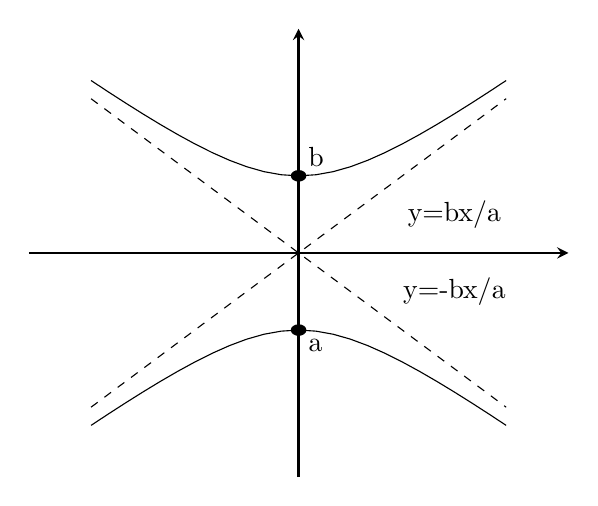
\begin{tikzpicture}
\begin{axis}[standard,domain=-4:4,xtick={\empty},ytick={\empty}]
\addplot[] {(x^2+4)^0.5};
\addplot[] {-(x^2+4)^0.5};
\addplot[dashed] {x};
\fill[] (0,2) circle [radius=0.15] node[above right]{b};
\node[] at (3,1) {y=bx/a};
\addplot[dashed] {-x};
\node[] at (3,-1) {y=-bx/a};
\fill[] (0,-2) circle [radius=0.15] node[below right]{a};
\end{axis}
\end{tikzpicture}
\end{center}


And we could solve this by paramaterizing the equation or using a substitution. Both hyperbolic.

\vspace{10pt}

We are definitely going to be expected to know hyperbolic properties, such as $\sinh2t=2\sinh t\cosh t$. These are similar to their trigonometric counterparts.

\end{document}